% $Header: /cvsroot/latex-beamer/latex-beamer/solutions/generic-talks/generic-ornate-15min-45min.en.tex,v 1.5 2007/01/28 20:48:23 tantau Exp $

%\documentclass[handout]{beamer}
\documentclass{beamer}
\usepackage{graphics}
\usepackage{ulem}
% This file is a solution template for:

% - Giving a talk on some subject.
% - The talk is between 15min and 45min long.
% - Style is ornate.



% Copyright 2004 by Till Tantau <tantau@users.sourceforge.net>.
%
% In principle, this file can be redistributed and/or modified under
% the terms of the GNU Public License, version 2.
%
% However, this file is supposed to be a template to be modified
% for your own needs. For this reason, if you use this file as a
% template and not specifically distribute it as part of a another
% package/program, I grant the extra permission to freely copy and
% modify this file as you see fit and even to delete this copyright
% notice.

%%%%%
% POUBELLE
%%%%%

%\begin{frame}{Zoom in image}
%\pgfdeclareimage[height=8cm]{orga}{img/organisation-Medical}
%  \framezoom<1><2>(0cm,0cm)(2cm,1.5cm)
%  \framezoom<1><3>(1cm,3cm)(2cm,1.5cm)
%  \framezoom<1><4>(3cm,2cm)(3cm,2cm)
%  \pgfuseimage{orga}
%\end{frame}

% image declaration
%\pgfdeclareimage[height=2cm]{analytics}{img/analytics}
%\pgfuseimage{analytics}
%\pgfdeclareimage[height=2cm]{liquidhandling}{img/liquidhandling}
%\pgfdeclareimage[height=2cm]{medical}{img/medical}
%\pgfdeclareimage[height=2cm]{robotics}{img/robotics}




\mode<presentation>
{
  \usetheme{Warsaw}
  % or ...
  	%\usecolortheme{seahorse} % handout
	%\usecolortheme{rose} % handout

  \setbeamercovered{transparent}
  
  	%\usepackage{pgfpages} % handout
	%\pgfpagesuselayout{2 on 1}[a4paper,border shrink=5mm] %handout
  % or whatever (possibly just delete it)
}

\usepackage[english]{babel}
% or whatever

\usepackage[latin1]{inputenc}
% or whatever

\usepackage{times}
\usepackage[T1]{fontenc}
% Or whatever. Note that the encoding and the font should match. If T1
% does not look nice, try deleting the line with the fontenc.

\title[HamMedIntern] % (optional, use only with long paper titles)
{Internship at HAMILTON MEDICAL}

\subtitle
{Testing a Medical Respirator} % (optional)

\author[ekeller]{Eric Keller\\ \texttt{ekeller@hamilton-medical.ch}}

%\author[Author, Another] % (optional, use only with lots of authors)
%{F.~Author\inst{1} \and S.~Another\inst{2}}
% - Use the \inst{?} command only if the authors have different
%   affiliation.

\institute[Universities of Somewhere and Elsewhere] % (optional, but mostly needed)
{
  %\inst{1}%
  EPITA \\
  (Ecole Pour l'Informatique et les Techniques Avancees)
}
   %\and
  %\inst{2}%
  %Department of Theoretical Philosophy\\
  %University of Elsewhere}
% - Use the \inst command only if there are several affiliations.
% - Keep it simple, no one is interested in your street address.

%\date[Short Occasion] % (optional)
\date
{\today / Final Presentation}

\subject{Talks}
% This is only inserted into the PDF information catalog. Can be left
% out.



% If you have a file called "university-logo-filename.xxx", where xxx
% is a graphic format that can be processed by latex or pdflatex,
% resp., then you can add a logo as follows:

\pgfdeclareimage[height=0.4cm]{logo-company}{company}
\logo{\pgfuseimage{logo-company}}

% Delete this, if you do not want the table of contents to pop up at
% the beginning of each subsection:
\AtBeginSubsection[]
{
  \begin{frame}<beamer>{Outline}
    \tableofcontents[currentsection,currentsubsection]
  \end{frame}
}


% If you wish to uncover everything in a step-wise fashion, uncomment
% the following command:

%\beamerdefaultoverlayspecification{<+->}


\begin{document}

\begin{frame}
  \titlepage
\end{frame}

\begin{frame}{Outline}
  \tableofcontents
  % You might wish to add the option [pausesections]
\end{frame}


% Since this a solution template for a generic talk, very little can
% be said about how it should be structured. However, the talk length
% of between 15min and 45min and the theme suggest that you stick to
% the following rules:

% - Exactly two or three sections (other than the summary).
% - At *most* three subsections per section.
% - Talk about 30s to 2min per frame. So there should be between about
%   15 and 30 frames, all told.

%------------------------------------------------------------------------------
\section{Introduction}

\subsection[Hamilton]{The Hamilton company}

\begin{frame}{Hamilton activities}
  % - A title should summarize the slide in an understandable fashion
  %   for anyone how does not follow everything on the slide itself.

\begin{columns}

  \column{.5\textwidth}
    \begin{block}{Liquid handling in life sciences}
      \begin{center}
	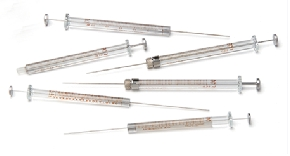
\includegraphics[height=2cm]{img/liquidhandling.jpg}
      \end{center}
    \end{block}

    \begin{block}{Life science robotics}
      \begin{center}
	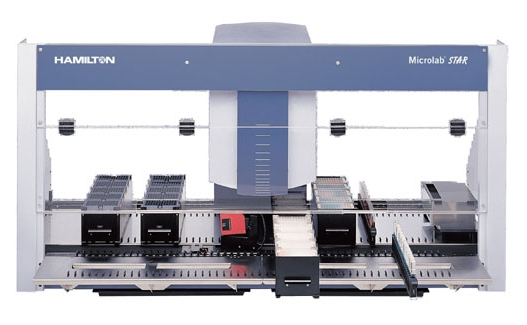
\includegraphics[height=2cm]{img/robotics.jpg}
      \end{center}
    \end{block}

  \column{.5\textwidth}
    \begin{block}{Analytics in life sciences}
      \begin{center}
	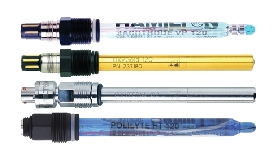
\includegraphics[height=2cm]{img/analytics.jpg}
      \end{center}
    \end{block}

    \begin{block}{Life support devices}
      \begin{center}
	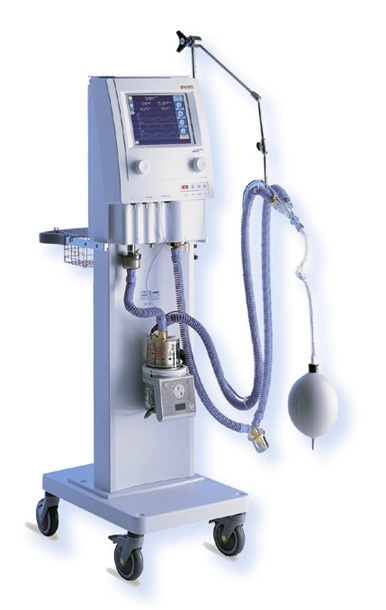
\includegraphics[height=2cm]{img/medical.jpg}
      \end{center}
    \end{block}
\end{columns}

\end{frame}

\begin{frame}{Key dates}
\begin{description}
\item[1947] Clark Hamilton, working from his garage at home, develops the first Hamilton syringe.
\item[1955] The success of Hamilton's products is enormous. Hamilton Co., US, is founded in Reno.
\item[1966] Hamilton's production facilities start to operate worldwide: HAMILTON BONADUZ AG.
\item[1983] HAMILTON MEDICAL AG is formed.
\end{description}

The Hamilton Group, a privately owned company employs approximately 1,000 people.
\end{frame}

\subsection[Organisation]{HAMILTON MEDICAL organisation}

\begin{frame}{New products}
  \begin{center}
    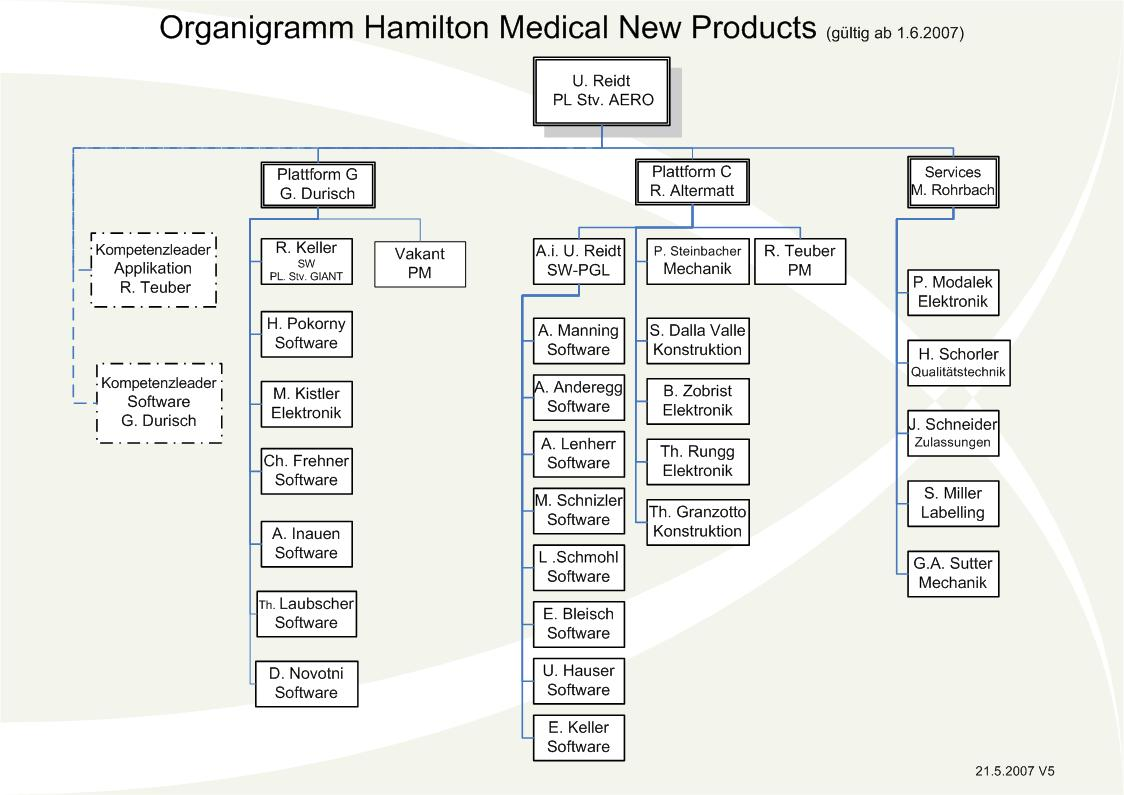
\includegraphics[height=7cm]{img/organisation-Medical.jpg}
  \end{center}
\end{frame}

\begin{frame}{The Nemo project}
The Nemo project is supervised by Roger Altermatt, my internship supervisor\\
The multidisciplinary Nemo team is composed of 14  people with experience in
these aeras:
\begin{itemize}
\item
  Modeling
\item
  Electronics
\item
  Software
\item
  Hardware
\end{itemize}

\end{frame}

%------------------------------------------------------------------------------
\section{Project status}

\begin{frame}{The Nemo project Timeline}
The Nemo project has been started in mid-2005.\\
When I joined the team the following were already developed:
  \begin{itemize}
    \item
      Nemo hardware prototype
    \item
      Nemo UML design defined in 3 layers
    \item
      70\% of the software functionalities
  \end{itemize}

But these had not yet been developed:

\begin{itemize}
\item
  The Nemo test concept
\item
  Module Test cases (Unit Tests)
\end{itemize}

\end{frame}

\subsection{Nemo Workspace}
\begin{frame}{The Nemo development tools}
The Nemo Project is developed on Microsoft Windows Host, using the following
software and hardware:
\begin{columns}
	\column{.5\textwidth}
	\begin{block}{Software Development}
	\begin{itemize}
		\item<1-> Telelogic Rhapsody 7.0
  		\item<2-> WindRiver Workbench 2.6
    \end{itemize}
    \end{block}

	\begin{block}{Other used tools}
	\begin{itemize}
      \item<3-> PVCS version manager
  	  \item<4-> EDO document manager
    \end{itemize}
    \end{block}

	\column{.5\textwidth}
	\begin{block}{Target Development}
	\begin{itemize}
      \item<5->WindRiver VxWorks 6.4
  	  \item<6-> Power PC 603
    \end{itemize}
    \end{block}
\end{columns}
\end{frame}

\subsection{Internship objectives}
\begin{frame}{Internship subject}
  \begin{block}{Initial subject}
    \alert{Test the Nemo project, a clinical respirator, against its technical specifications}
  \end{block}
  \begin{block}{Subject details}
    \begin{itemize}
    \item<1-> Elaboration of the test concept.
    \item<2-> Testing the code of critical modules.
    \item<3-> Testing the Rhapsody framework generated code.
    \item<4-> System testing
    \end{itemize}
  \end{block}
\end{frame}

\subsection{Testing knowledge}

\begin{frame}{How should we test a software}
\begin{center}
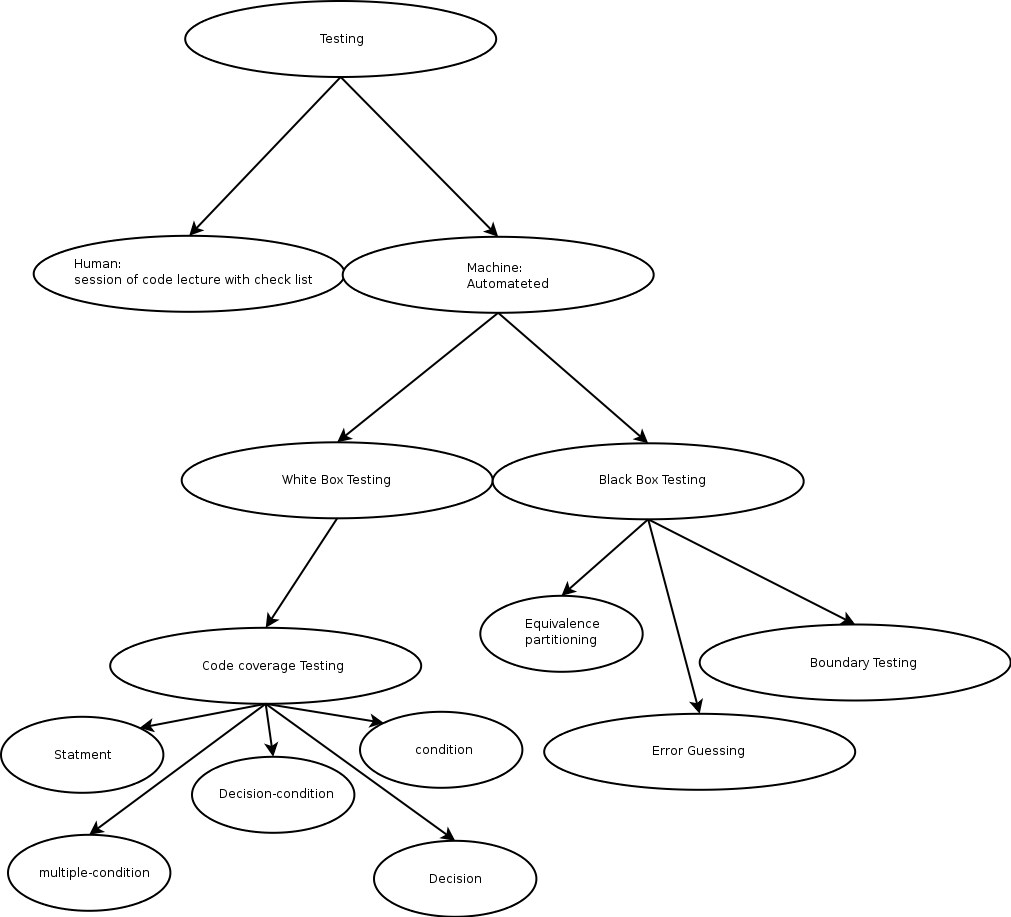
\includegraphics[height=7cm]{img/SoftTesting.png}
\end{center}
\end{frame}

\begin{frame}{Software testing concept}

Common \alert{misconceptions} about testing are:
\begin{definition}
  \begin{itemize}
    \item<1->
      \uwave{Testing is the process of demonstrating that errors are not present.}
    \item<2->
      \uwave{The purpose of testing is to show that a program performs its intended functions correctly.}
   \end{itemize}
\end{definition}
A more appropriate definition would be\cite{Glenford04}:
\begin{definition}
  Testing is the process of executing a program\\
  with the intent of finding errors.
\end{definition}
\end{frame}

\begin{frame}{Medical norm and FDA requirements}
  \begin{columns}

    \column{.5\textwidth}
    \begin{block}{FDA\cite{FDA02}}
    \begin{itemize}
      \item Preliminary risk analysis.
      \item Traceability analysis
      \item System test plan generation
      \item Acceptance test plan generation
      \item Code coverage
    \end{itemize}
    \end{block}

    \column{.5\textwidth}
    \begin{block}{European Medical Norm\cite{IEC06}}
    \begin{itemize}
      \item Determining risk
      \item Safety classification
      \item SW unit implementation and verification
    \end{itemize}
    \end{block}

  \end{columns}
\end{frame}

%------------------------------------------------------------------------------
\section{Realisations}

\subsection{Prerequisite}
\begin{frame}{Evaluation of the available test tools}
Several test tools were available:
\begin{description}
  \item[Unit Tester] is the WindRiver Workbench Module test tool (based on IPL Cantata product).
  \item[Test Conductor] is the Ilogix Rhapsody integrated test tool.
  \item[ATG] (Automatic Test Generator) is a Rhapsody integrated test tool.
  \item[Cpp Unit] is a free C++ unit testing framework.
  \item[Polyspace] provides the first and only exhaustive code analysis detecting run-time errors.
\end{description}
\end{frame}

\begin{frame}{WindRiver UnitTester choice}
The WindRiver UnitTester was chosen for the following reasons:
\begin{itemize}
\item<1-> Code coverage
\item<2-> Pre-existing knowledge and experience (WindRiver Workbench already in
use for debugging)
\item<3-> IPL Cantata++ Knowledge
\item<4-> UnitTester being used by other HAMILTON MEDICAL ventilator development
team
\item<5-> Price and availability
\end{itemize}
\end{frame}

\begin{frame}{Testing Nemo}
These are the testing phases we planned for the Nemo project:
\begin{enumerate}
\item Static tests
\item Unit tests
\item Integration tests
\item System tests
\end{enumerate}
\end{frame}

\subsection{The Nemo test concept}

\begin{frame}{Designing the Nemo test concept}
\begin{itemize}
  \item<1-> Regulatory drivers
  \item<2-> Workflow
	\begin{itemize}
  		\item Coverage and boundary tests
  		\item Functionality tests
  		\item Stress tests
  		\item Robustness tests
  		\item Functionality tests
  	\end{itemize}
  \item<3-> Test prerequisites
  \item<4-> Definition of test cases
	\begin{itemize}
	  \item Real time and multitasking test scenarios
	  \item Test evolution
	  \item Automatic checking
	\end{itemize}
  \item<5-> Road Map
	\begin{itemize}
  		\item Module criticality
  		\item Milestones
  	\end{itemize}
\end{itemize}
\end{frame}

\begin{frame}{Adapting the development workflow}
  \begin{center}
    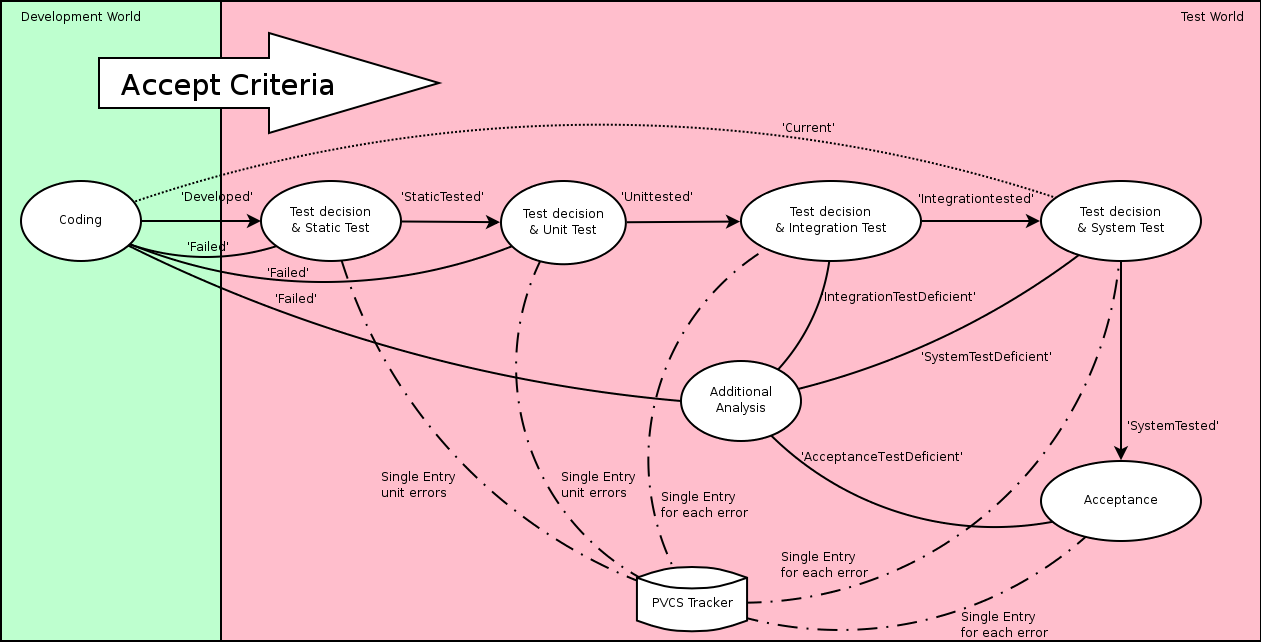
\includegraphics[height=6cm]{img/TestWorkflow.png}
  \end{center}
\end{frame}

\begin{frame}{Enabling the testing workflow}
  \begin{columns}

    \column{.5\textwidth}
    \begin{block}{Previous workflow}
      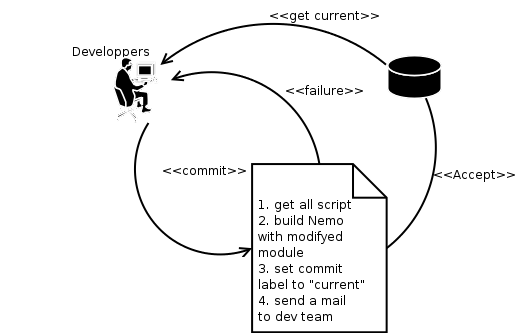
\includegraphics[height=3.5cm]{img/workflow.png}
    \end{block}

    \column{.5\textwidth}
    The testing workflow adds the following steps
    \begin{enumerate}
    \item<1-> Submits the model to the test world
    \item<2-> Sets a time stamp label over the source, model, bsp, \ldots
    \end{enumerate}
  \end{columns}
\begin{description}
 \item<3->[The results] of those additional steps are an identifiable software
\end{description}
\end{frame}

\begin{frame}{Scripting}
The Nemo project use a lot of batch scripts for building the software.\\
For applying the test concept I introduced the \alert{Perl} scripting language,\\
far more adapted to realise the test Workflow.

\end{frame}

\subsection{Problems and solutions}

\begin{frame}{Rhapsody / WindRiver interaction}
Practically all problems encountered resulted from tool interaction.\\
Combining Telelogix Rhapsody and WindRiver Workbench caused the following 
problems:
\begin{columns}
    \column{.5\textwidth}
    \begin{block}{Problems}
      \begin{itemize}
      \item Makefile process
      \item Compiler options
      \item Includes and link libraries
      \item Rhapsody framework
      \end{itemize}
    \end{block}

    \column{.5\textwidth}
    \begin{block}{Solutions}
      \begin{itemize}
      \item Adapting the makefile to our needs
      \item Generating additional makefile
      \item Framework workshop
      \end{itemize}
    \end{block}
\end{columns}
\end{frame}

\begin{frame}{UnitTester with C++}

\begin{columns}

\column{.5\textwidth}
\begin{block}{Problems}
  \begin{itemize}
  \item Bad documentation and tutorial
  \item Code instrumentation fails with Rhasody generated code
  \item Call sequence segfault with multithreaded test cases
  \item Test template generation of Stub or Wrapper will not compile
  \end{itemize}
\end{block}

\column{.5\textwidth}
\begin{block}{Solution}
  \begin{itemize}
  \item development of an internal Cookbook
  \item Upgrade to 2.6 version
  \item Intense communication with IPL support
  \end{itemize}
\end{block}
\end{columns}
\end{frame}

\begin{frame}{Source versioning with PVCS}
We had to develop several workaround for using the PVCS version control manager:
\begin{itemize}
\item Labeling the code and models
\item Using an old version of the program
\item Misdocumented commands
\end{itemize}
\end{frame}

%\subsection{Further steps}

%\begin{frame}{Begining of the Integration / System Test}
%\end{frame}


%------------------------------------------------------------------------------
\section*{Summary}

\begin{frame}{Summary}

  % Keep the summary *very short*.
  \begin{itemize}
  \item
    \alert{Software Testing} is is an extremely creative and intellectually 
    challenging task.
  \item
    Software Testing is \alert{not} limited to Black Box Testing.
  \end{itemize}
\end{frame}

\begin{frame}{Conclusion}
During my internship at HAMILTON MEDICAL I acquired several competencies
\begin{itemize}
\item New point of view about software testing
\item Medical exigences (Norms)
\item Improvement of my German
\item Aquaintance with Quality activities
\item Experience with a team organisation
\end{itemize}
\end{frame}

% bibliographie

\begin{frame}{Further lectures}
\begin{thebibliography}{10}
\bibitem{Glenford04}[Glenford, 2004]
  Glenford J. Myers.
  \newblock The Art Of Software Testing
  \newblock provides a practical discussion of the purpose and nature of software testing, offering the latest methodologies for the design of effective test cases.

\bibitem{IEC06}[IEC, 2006]
IEC. International Standard Medical device software - Software life cycle processes.
\newblock IEC, 2006. This reference Norm present all the points to confom to the Norm ISO-62304. It defines the risk and how to prevent them.

\bibitem{FDA02}[FDA, 2002]
\url{www.fda.gov}
\newblock U.S. Department of health and Human Services. Introduce general principles of software validation.

\end{thebibliography}
\end{frame}


\appendix
\section{\appendixname}
\begin{frame}{Outline}
	\tableofcontents
\end{frame}


\subsection{Additional material}

\begin{frame}{Develoment and test cycle}
\begin{center}
    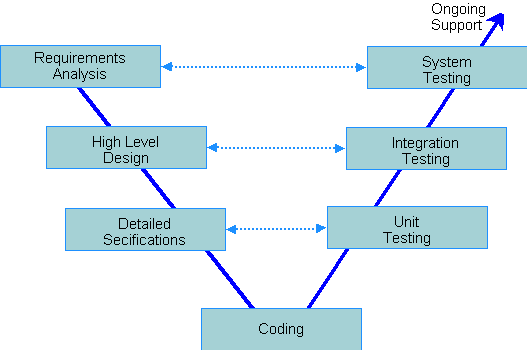
\includegraphics[height=6cm]{img/VCycleNemo.png}
  \end{center}
\end{frame}

\begin{frame}{Generation of UnitTester project}
\begin{center}
    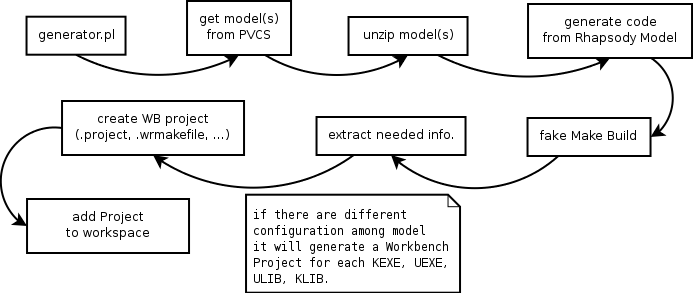
\includegraphics[height=4cm]{img/UTProject_generator_toolchain.png}
  \end{center}
\end{frame}

\begin{frame}{Rhapsody vs. Workbench}
\begin{center}
    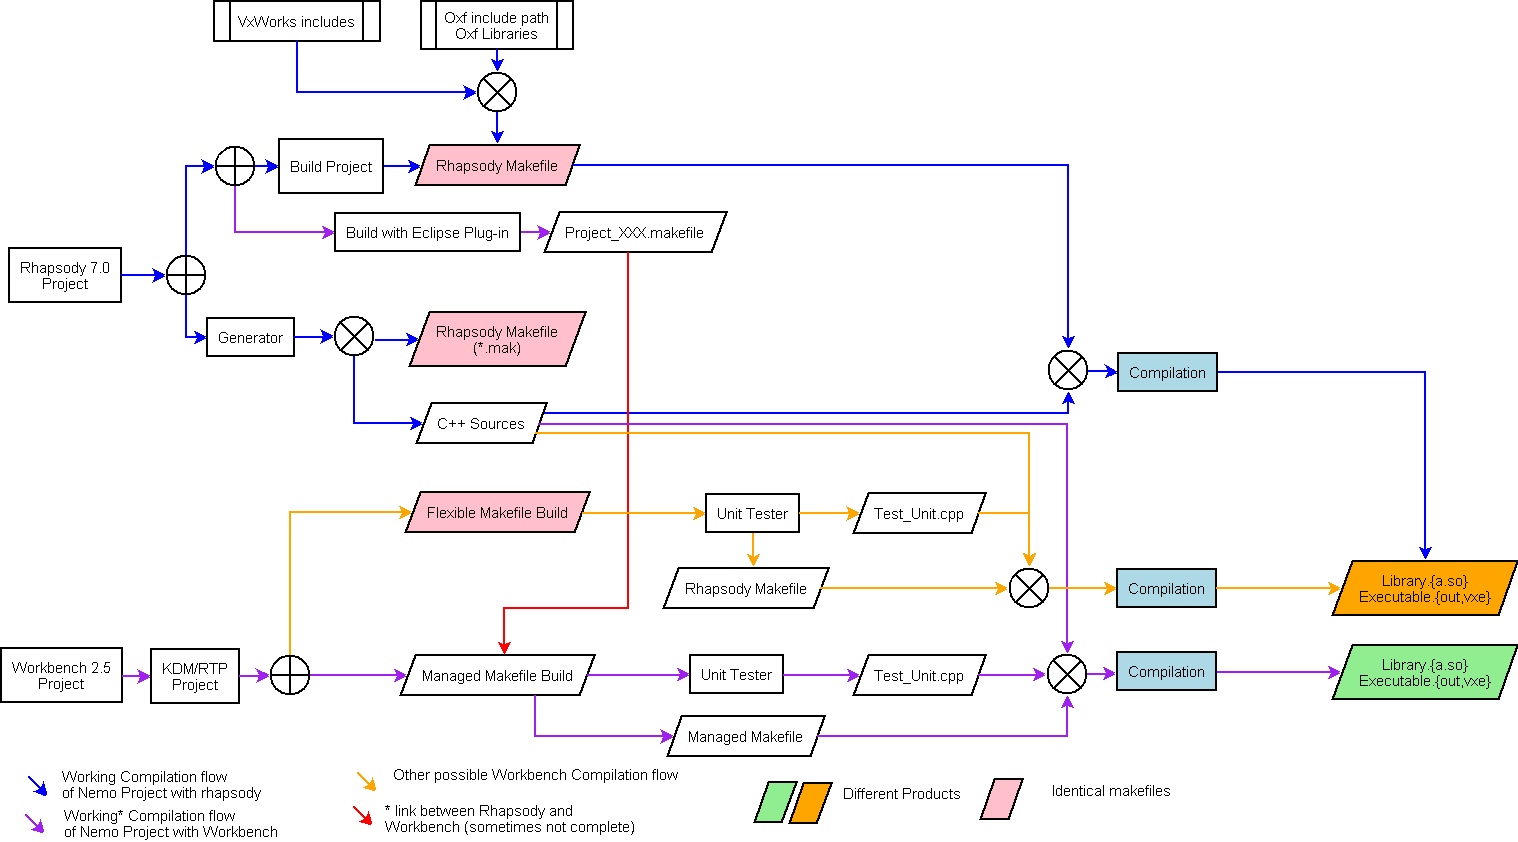
\includegraphics[height=6cm]{img/RHWB.png}
 \end{center}
\end{frame}

\subsection{Testing examination}

\begin{frame}{The triangle test\cite{Glenford04}}
\begin{definition}
Imagine a program reading three integer values from an input dialog. The
three values represent the lengths of the sides of a triangle. The
program displays a message that states whether the triangle is scalene,
isosceles, or equilateral.
\end{definition}

Let's elaborate test cases for this progam\ldots

\end{frame}

\begin{frame}{Solution}
Do you have:
\begin{columns}
	\column{.5\textwidth}
	\begin{itemize}
      \item a test case that represents a valid scalene triangle? \alert{test cases
      such as 1,2,3 and 2,5,10 are not triangle}
      \item a test case that represents a valid equilateral triangle?
      \item a test case that represents a valid isosceles triangle? \alert{a
      test case representing 2,2,4 is not a valid triangle}     
    \end{itemize}
	\column{.5\textwidth}
	\begin{itemize}
      \item Do you have a test case in which one side has a zero value?
      \item Do you have a test case in which one side has a negative value?
      \item Do you have a test case with three integers greater than zero such
      that the sum of two of the numbers is equal to the third?
    \end{itemize}
\end{columns}
\end{frame}

\begin{frame}{Solution 2}
Do you have:
\begin{columns}
	\column{.5\textwidth}
	\begin{itemize}
      \item at least three test cases that represent valid isosceles triangles
      such that you have tried all three permutations of two equal sides (such as, 3,3,4; 3,4,3; and 4,3,3)?      
	  \item Do you have at least one test case specifying the wrong number of arguments
    \end{itemize}
	\column{.5\textwidth}
	\begin{itemize}
      \item Do you have a test case with three integers greater than zero such
      that the sum of two of the numbers is less than the third (such as 1,2,4
      or 12,15,30)?
      \item a test case for all three permutations for the previous point
    \end{itemize}
\end{columns}
\end{frame}


\end{document}


